\documentclass[norsk, a4paper]{article}

\usepackage[T1]{fontenc}    % Riktig fontencoding
\usepackage[utf8]{inputenc} % Riktig tegnsett
\usepackage{babel}          % Ordelingsregler, osv
\usepackage{graphicx}       % Inkludere bilder
\usepackage{booktabs}       % Ordentlige tabeller
\usepackage{url}            % Skrive url-er
\usepackage{textcomp}       % Den greske bokstaven micro i text-mode
\usepackage{units}          % Skrive enheter riktig
\usepackage{float}          % Figurer dukker opp der du ber om
\usepackage{lipsum}         % Blindtekst
\usepackage{amsmath}        % math

% JF i margen
\makeatletter
\renewcommand{\subsubsection}{\@startsection{subsubsection}{3}{-2cm}%
{-\baselineskip}{0.5\baselineskip}{\bf\large}}
\makeatother
\newcommand{\jf}[1]{\subsubsection*{JF #1}\vspace*{-2\baselineskip}}

% Skru av seksjonsnummerering
\setcounter{secnumdepth}{-1}

\begin{document}

% Forside
\begin{titlepage}
\begin{center}

\textsc{\Large FYS3220 - Lineær kretselektronikk}\\[0.5cm]
\rule{\linewidth}{0.5mm} \\[0.4cm]
{ \huge \bfseries  LABORATORIEØVELSE A}\\[0.10cm]
\rule{\linewidth}{0.5mm} \\[1.5cm]

\textsc{\Large Fourieranalyse}\\[1.5cm]

% Av hvem?
\begin{minipage}{0.49\textwidth}
    \begin{center} \large
        Snorre Bjørnstad (snorrebj)\\ \url{snorrebj@student.matnat.uio.no} \\[0.8cm]
        %\includegraphics{bilde1}
    \end{center}
\end{minipage}
\begin{minipage}{0.49\textwidth}
    \begin{center} \large
        Arne Johan Bergli (ajbergli)\\ \url{ajbergli@student.matnat.uio.no} \\[0.8cm]
        %\includegraphics{bilde2}
    \end{center}
\end{minipage}

\vfill

% Litt info nederst
\large{
\begin{tabular}{r@{: }l}
Labdag & XX \\
Dato & \today
\end{tabular}
}

\end{center}
\end{titlepage}

\section{Oppgave 1: Summering av signaler}
\jf{1.a}
\begin{figure}
 \begin{center}
   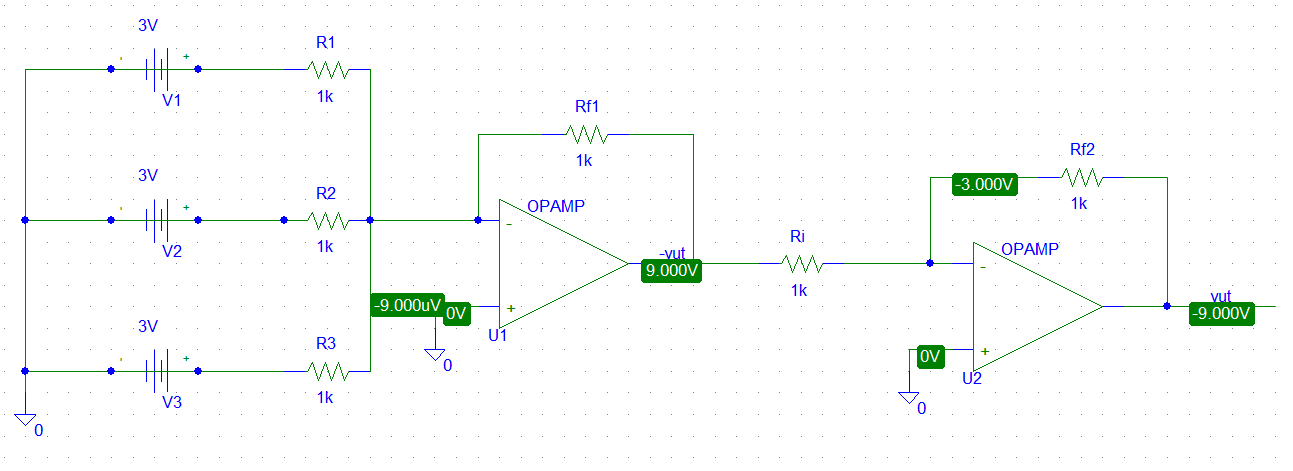
\includegraphics[width=1\textwidth]{Figurer/oppg1_schem.PNG}\\
   \caption{\textit{Summeringskretsen for oppgave 1a}}\label{fig:oppg1_schem}
 \end{center}
\end{figure}


\section{Oppgave 2: Simulering av egen blanding av frekvenskomponenter}
\jf{2.a}

\begin{align*}  v(t)&=0\\ &+ 1\cdot\sin{(2\pi\cdot 500Hz)}\\ &+ 0.5 \cdot \sin{(2\pi\cdot 1000Hz)}\\ &+ 0.6 \cdot \sin{(2\pi\cdot 1300Hz)}\\ &+ 0.4 \cdot \sin{(2\pi\cdot 1900Hz)}\\ & + 0.2 \cdot \sin{(2\pi\cdot 3000Hz)}\end{align*}

\jf{2.b}


\jf{2.c}
\lipsum[1]

\section{Oppgave 3: dc og $b_n$ for $v(t)$}
\jf{3.a}
\lipsum[1]

\jf{3.b}
\lipsum[1]

\section{Oppgave 4: Studie av Fourierspekteret til en firkantserie}
\jf{4.a}
\begin{table}[H]
  \centering
  \begin{tabular}{ l r r p{2cm} p{1.3cm} p{1.4cm} p{1.4cm} }
    \toprule
    & $n$ & $a_n$ & \centering $b_n$ Beregnet \par [V] & $b_n$ Målt \par [mV] &
    Frekvens \par [kHz] & Vinkelf. \par [rad/s] \\
    \midrule
     DC-verdi     &  0 & 0 & & & & \\
     Grunntone    &  1 & 0 & & & & \\
     2-Harmoniske &  2 & 0 & & & & \\
     3-Harmoniske &  3 & 0 & & & & \\
     4-Harmoniske &  4 & 0 & & & & \\
     5-Harmoniske &  5 & 0 & & & & \\
     6-Harmoniske &  6 & 0 & & & & \\
     7-Harmoniske &  7 & 0 & & & & \\
     8-Harmoniske &  8 & 0 & & & & \\
     9-Harmoniske &  9 & 0 & & & & \\
    10-Harmoniske & 10 & 0 & & & & \\
    \bottomrule
  \end{tabular}
  \caption{Teoretisk beregnede og målte komponenter for et oddesymmetrisk
  firkantsignal}
  \label{tab:komponenter_firkant}
\end{table}

\jf{4.b}
\lipsum[1]

\section{Oppgave 5: Rekonstruksjon av et firkantsignal}
\jf{5.a}
\lipsum[1]

\section{Oppgave 6: Studie av spekteret til et firkantsignal når periodetiden
øker}
\jf{6.a}
\lipsum[1]

\jf{6.b}
\lipsum[1]

\section{Oppgave 7: Studie av spekteret til en firkantpuls som har avtakende
pulsbredde}
\jf{7.a}
\begin{table}[H]
  \centering
  \begin{tabular}{r c}
    \toprule
    Pulsbredde [\unit{\textmu s}] & Båndbredde [kHz]\\
    \midrule
    $ 1000 $ & \\
    $ 100  $ & \\
    $ 30   $ & \\
    $ 10   $ & \\
    $ 3    $ & \\
    $ 1    $ & \\
    \bottomrule
    \end{tabular}
  \caption{Sammenheng mellom pulsbredde og båndbredde for en firkantpuls med
  periode på 1000 ms}
  \label{tab:bandwidth}
\end{table}

\jf{7.b}
\lipsum[1]

\jf{7.c}
\lipsum[1]

\jf{7.d}
\lipsum[1]

\section{Oppgave 8. Studie av frekvensspekteret til en ekte sagtann}

\jf{8.a}
\begin{table}[H]
  \centering
  \begin{tabular}{l r p{1.7cm} p{1.9cm} p{1.9cm} p{1.5cm}}
    \toprule
    & $n$ & $b_n$ Firkant \par [mV] & $b_n$ Sagtann1 \par [mV]
    & $b_n$ Sagtann2 \par [mV] & Frekvens \par [kHz] \\
    \midrule
     DC verdi     &  0 & & & & \\
     Grunntone    &  1 & & & & \\
     2-Harmoniske &  2 & & & & \\
     3-Harmoniske &  3 & & & & \\
     4-Harmoniske &  4 & & & & \\
     5-Harmoniske &  5 & & & & \\
     6-Harmoniske &  6 & & & & \\
     7-Harmoniske &  7 & & & & \\
     8-Harmoniske &  8 & & & & \\
     9-Harmoniske &  9 & & & & \\
    10-Harmoniske & 10 & & & & \\
    \bottomrule
  \end{tabular}
  \caption{Sammenheng mellom frekvenskomponentene til et firkant- og
  sagtannsignal}
  \label{tab:komponenter_sagtann}
\end{table}

\jf{8.b}
\lipsum[1]

\section{Oppgave 9. Studie av tilnærmingsfunksjon for en ekte sagtann}
\jf{9.a}
\lipsum[1]

\section{Oppgave 10. Studie av fase for sagtannsignal}
\jf{10.a}
\lipsum[1]

\jf{10.b}
\lipsum[1]

\end{document}
